\documentclass[aps,pra,reprint,superscriptaddress,nofootinbib]{revtex4-2}
\usepackage{amsmath,amssymb,graphicx,bm}
\usepackage{booktabs}
\usepackage{amsthm}
\newtheorem{proposition}{Proposition}

\begin{document}

\title{Which quantum algorithms suit photonic continuous-variable hardware?
A comparative resource and noise-robustness study}

\author{Hikaru Wakaura}
\author{Taiki Tanimae}
\affiliation{QIRI (Quantum Integrated Research Institute Inc.),
1--16--3, Akasaka, Minato-ku, Tokyo 107--0061, Japan.\\
Correspondence:\ h.wakaura@deeptell.jp
(ORCID 0000-0001-8381-8323), t.tanimae@deeptell.jp} 
 
\date{\today} 

\begin{abstract}  
Photonic continuous-variable (CV) processors offer a deterministic route
to scalable quantum computing, but the cost of fault tolerance depends
strongly on how a given algorithm uses non-Gaussian resources and circuit
depth. It is not known, across representative algorithm classes, which are
intrinsically robust on CV hardware and how much Gottesman--Kitaev--Preskill
(GKP) error correction helps. Here we port four algorithms---control-free
quantum phase estimation (QPE), randomized product formulas (qDRIFT), quantum
Kolmogorov--Arnold networks (QKAN), and Regev's factoring algorithm---to a
common CV model and compare them under a shared noise channel combining
photon loss and Gaussian displacement. Across the tested algorithm classes and
noise regime, we find that control-free QPE is the most noise-robust because it
requires no controlled unitaries and, for quadratic Hamiltonians, no
non-Gaussian gates---a property that survives for non-Gaussian Hamiltonians. We
show analytically and numerically that GKP correction helps only once the
physical noise exceeds the finite-squeezing floor, and that whether an
algorithm gains from correction is set by a noise- versus systematic-limited
dichotomy: deep, noise-sensitive algorithms (QKAN, Regev) gain most (up to
$\sim\!2.7\times$ at $18$~dB, an optimistic bound under our loss model), while
shallow QPE stays near its clean floor and needs little correction. This is a
model-level comparative study, not an experiment; its value is a unit-robust
ranking with sensitivity analysis and analytic statements that turn the
folklore ``minimize non-Gaussian resources and depth'' into quantitative,
testable criteria for algorithm selection on near- and intermediate-term
photonic devices.
\end{abstract} 
 
\maketitle

\section{Introduction} 
Simulating and computing with quantum systems is among the most promising
applications of quantum computers. Photonic continuous-variable (CV)
architectures encode information in the quadratures of bosonic
modes~\cite{Lloyd1999,Braunstein2005,Weedbrook2012} and support
deterministic, room-temperature generation of large cluster
states~\cite{Larsen2019,Asavanant2019,Madsen2022}, making them a leading
candidate for scalable fault-tolerant quantum computing. Fault tolerance on
CV hardware is provided by bosonic codes, most prominently the
Gottesman--Kitaev--Preskill (GKP) code~\cite{GKP2001}, whose overhead is set
by the achievable squeezing and by the number of non-Gaussian resource
states consumed~\cite{Albert2018,Cochrane1999,Michael2016,Tzitrin2021,
Noh2020,Pantaleoni2020}.

Different algorithms place very different demands on this substrate. Some
require controlled unitaries (hard on CV because they need a clean control
mode and high non-Gaussianity~\cite{Bartlett2002,Eisert2002}); some are
dominated by non-Gaussian gate count; some by circuit depth. However, no
unified comparison exists that quantifies, across representative algorithm
classes, which algorithms are intrinsically robust on CV hardware and how
much GKP error correction improves them. In this
study, we port four representative algorithms to a common CV model and compare
them under a shared noise channel. We find that control-free QPE is the most
noise-robust and benefits most from GKP correction, and we derive a depth-
limited correction law and a finite-squeezing threshold for when correction
helps.

\paragraph{Relation to prior work.}
CV measurement-based fault tolerance and GKP-encoded cluster states have been
developed extensively~\cite{Menicucci2014,Bourassa2021,Fukui2018,Walshe2020,
Terhal2020,Konno2024}, and the Gaussian no-go theorem~\cite{Niset2009}
establishes that non-Gaussian resources are mandatory for correcting Gaussian
errors. Quantum signal processing and singular-value transformation provide
a unified framework for many algorithms~\cite{Low2017,Gilyen2019,Rossi2022}. Our contribution is not a new algorithm or a new code,
but the first \emph{cross-algorithm} CV resource-and-noise comparison on a
common footing, together with three analytic statements
(Propositions~\ref{prop:floor}--\ref{prop:regev}) that explain the observed
ordering. We are explicit (Sec.~\ref{sec:limits}) about which results are
exact, which are model-level surrogates, and which are extrapolations.

\section{CV mapping framework}
We map each algorithm onto bosonic modes encoded, where fault tolerance is
required, in GKP qubits. Gaussian operations (interferometers, squeezers,
phase rotations) are treated as inexpensive; non-Gaussian gates such as the
cubic-phase gate~\cite{Marek2011,GKP2001} and GKP magic
states~\cite{Eaton2019,Konno2024} are the costly resource, analogous to the
$T$-count in discrete-variable (DV) circuits. This reflects the Gaussian
no-go theorem~\cite{Niset2009,Eisert2002}.

The four algorithms are chosen to span the axes that govern CV cost:
controlled-unitary requirement (QPE: none; Regev: heavy), non-Gaussian gate
density (QKAN: high; QPE-quadratic: zero), circuit depth (Regev: deep; QPE:
shallow), and task type (Hamiltonian simulation, spectroscopy, machine
learning, number theory). They are illustrative rather than exhaustive; we do
not claim coverage of all CV algorithms.

\section{Algorithm ports}
\subsection{Control-free QPE}
The time series $f(t)=\langle\psi|e^{iHt}|\psi\rangle$ is acquired without
controlled unitaries; the spectrum is recovered by reference-eigenstate
holographic phase retrieval, drawing on classical phase-retrieval
techniques~\cite{Fienup1982}. The control-free protocol is due to Clinton
\emph{et al.}~\cite{Clinton2026}, generalizing the standard QPE
construction~\cite{Kitaev1995}; our contribution is the CV-specific
observation and
quantification that, for quadratic $H$, $e^{iHt}$ is purely Gaussian, so the
entire circuit needs \emph{zero} controlled unitaries and \emph{zero}
non-Gaussian gates---uniquely matching the CV cost structure---and that this
advantage \emph{survives} for non-Gaussian $H$ (Sec.~\ref{sec:nong}), where
only the cost of a non-Gaussian Trotterized $e^{iHt}$ is added while the
control-free property is retained.

\subsection{qDRIFT}
$H=\sum_l h_l$ is written as a sum of bosonic terms; importance-sampled
product formulas approximate $e^{-iHt}$~\cite{Campbell2019}, with the
number of steps $N$ independent of the number of terms $L$. Sharper
concentration bounds for single realizations are due to Chen, Huang, Kueng
and Tropp~\cite{Chen2021}; these results are complementary to deterministic
Trotter analyses~\cite{Berry2015,Childs2021}.

\subsection{QKAN}
Quantum singular value transformation~\cite{Low2017,Gilyen2019} is realized
through bosonic quantum signal processing~\cite{Rossi2022}: Chebyshev
polynomials $T_r(x)=\cos(r\arccos x)$ are the natural phase-space-rotation
response. QKAN~\cite{Ivashkov2024} ports the classical Kolmogorov--Arnold
architecture~\cite{Liu2024} into this framework.

\subsection{Regev factoring}
Regev's factoring algorithm~\cite{Regev2023}, an asymptotic refinement of
Shor's algorithm~\cite{Shor1997} with $\tilde O(n^{3/2})$ gates,
prepares the discrete Gaussian state
$\rho_R(z)\propto e^{-\pi z^2/R^2}$, which we identify with a
finite-energy GKP comb. The QFT becomes a mode-wise CV-QFT; modular
exponentiation runs on GKP qubits and is the rate-limiting non-Gaussian
step. Qubit-efficient Shor variants~\cite{Beauregard2003} would inherit
the same non-Gaussian arithmetic bottleneck on CV.
We verify correctness end-to-end on six biprimes ($143$--$391$): the CV
quantum core feeds classical LLL post-processing and recovers a factor with
$100\%$ success over $5$ seeds each. We stress that the naive GKP-comb readout
demands squeezing growing as $\sqrt{n}$ (Prop.~\ref{prop:regev}), which is
\emph{prohibitive} for cryptographic $n$; we therefore present Regev as a
worked correctness demonstration and a cautionary resource case, not as a
practical CV factoring route. The lattice-spacing rescaling that would relax
this requirement is left as an explicit open problem.

\section{Methods}\label{sec:methods}
\emph{GKP logical error model.} The per-quadrature logical flip probability
under a residual displacement of std $\sigma$ is
$p_{\rm round}=1-\mathrm{erf}\!\big(\tfrac{\sqrt\pi/2}{\sqrt2\,\sigma_{\rm eff}}\big)$
with $\sigma_{\rm eff}^2=\sigma^2+\Delta^2$, and
$p_L=1-(1-p_{\rm round})^{2}$ for the two quadratures; this is the standard
single-round GKP shift-error model~\cite{GKP2001,Glancy2006} and the source
of $p_L$ used above. We
emphasize two scope points. (i)~$p_L$ is a \emph{single-round} logical error
rate; it is not the fault-tolerant threshold (which for concatenated GKP is
$\sim10$~dB), and our ``dB'' axis should be read as the physical squeezing
setting the floor $\Delta$, not as a threshold statement. (ii)~Photon loss is
corrected here only through its leading-order displacement-equivalent variance;
a full loss correction additionally requires
amplification~\cite{Albert2018,Noh2020,Walshe2020} and is expected to
\emph{raise} the squeezing needed, so our GKP improvement factors under loss
are \emph{optimistic bounds} on what single-round, displacement-only GKP
achieves.
\emph{Statistics.} All stochastic quantities use $10$ seeds; we report means
with $95\%$ confidence intervals $1.96\,\hat\sigma/\sqrt{10}$. Improvement
factors $r=u/c$ are reported with propagated relative uncertainty
$\delta r/r=\sqrt{(\delta u/u)^2+(\delta c/c)^2}$; values quoted as ``$\times k$''
have $\delta r/r\lesssim 15\%$ unless noted.
\emph{Simulation.} Loss and displacement are exact Fock-space channels;
Hamiltonian evolution uses exact diagonalization or precomputed step
unitaries. \emph{Reproducibility.} Each port is a standalone script
(\texttt{qpe\_cv.py}, \texttt{qdrift\_cv.py}, \texttt{qkan\_cv.py},
\texttt{regev\_cv.py}); the cross comparison is \texttt{noise\_comparison.py};
the GKP-model validation is \texttt{gkp\_validate.py}; the 2D phase diagram and
ensembles are \texttt{noise\_phase\_diagram.py}; the DV baseline is
\texttt{dv\_baseline.py}; figures are generated by \texttt{make\_figs.py} from
the released JSON results. Every figure and table maps to one such artifact.

\section{Results}
\subsection{Noise model and GKP correction}
Per noise-exposed operation we apply photon loss (transmissivity $\eta$) as
an \emph{exact} Fock-space Kraus channel,
$E_l=\sqrt{(1-\eta)^l/l!}\,\eta^{\hat n/2}a^l$, and Gaussian displacement
(std $\sigma_d$) as an exact unitary kick. The two channels are simulated
exactly in their respective ports; the dynamical evolution is therefore not
approximated. Only for the \emph{GKP residual-noise model} do we summarize the
combined channel by an equivalent displacement variance
$\sigma_{\rm loss}^2=(1-\eta)/2$ (the vacuum variance injected to leading
order); this is a deliberate surrogate, valid in the small-loss regime and
flagged in Sec.~\ref{sec:limits}, used only to parametrize
$\sigma_{\rm corr}^2=(1-p_L)\Delta^2+p_L\sigma_{\rm phys}^2$, where
$\sigma_{\rm phys}^2=\sigma_d^2+\sigma_{\rm loss}^2$, $\Delta(\mathrm{dB})$ is
the finite-squeezing peak width and $p_L$ the GKP logical error rate. Loss-
\emph{induced} dynamics in each algorithm are computed from the true Kraus
channel, not from this surrogate. The surrogate itself is validated against an
explicit GKP EC-protocol Monte Carlo in Sec.~\ref{sec:valid}
(agreement $\le0.1\%$).

\subsection{Validation of the GKP correction model}\label{sec:valid}
To establish that our conclusions do not rest on an unverified assumption, we
validate the surrogate against an explicit Monte-Carlo simulation of the
single-round GKP error-correction protocol~\cite{Glancy2006,GKP2001}: input
shift
$e\sim\mathcal N(0,\sigma_{\rm phys})$, finite-squeezing ancilla syndrome noise
$\xi\sim\mathcal N(0,\Delta)$, modular measurement
$s=\mathrm{wrap}_{\sqrt\pi}(e+\xi)$, correction, and logical-error detection
(Table~\ref{tab:valid}). Three checks pass: (i)~the analytic per-quadrature
logical error $p_{\rm round}$ matches the explicit protocol to within absolute
$3\times10^{-4}$ over $\sigma_{\rm phys}\in[0.1,0.4]$, dB$\in\{9,12,15\}$
(relative agreement $\le16\%$ only at the smallest $p\sim10^{-3}$, limited by
Monte-Carlo sampling); (ii)~the post-correction continuous residual equals the
finite-squeezing floor, $\sigma_{\rm res}/\Delta=1.00$; (iii)~the scalar
surrogate $\sigma_{\rm corr}$ matches the explicit two-channel
(floor-$\Delta$ plus logical-rate-$p_L$) model to within $0.1\%$. The core GKP
model is therefore validated, not assumed.

\begin{table}[t]
\caption{Validation of the GKP correction model against an explicit EC-protocol
Monte Carlo (excerpt; $10$ seeds, $2\times10^5$ samples each).}
\label{tab:valid}
\begin{tabular}{lccc}
\toprule
quantity & analytic/surrogate & explicit MC & agreement\\
\midrule
$p_{\rm round}$ ($\sigma{=}0.3$, 12\,dB) & $0.0110$ & $0.0109$ & $1.0\%$\\
$p_{\rm round}$ ($\sigma{=}0.4$, 9\,dB) & $0.0605$ & $0.0603$ & $0.4\%$\\
residual $\sigma_{\rm res}/\Delta$ & $1$ & $1.00$ & exact\\
$\sigma_{\rm corr}$ (all cases) & --- & --- & $\le0.1\%$\\
\bottomrule
\end{tabular}
\end{table}

\subsection{Noise robustness}
Table~\ref{tab:robust} reports the robustness onset. Control-free QPE keeps
its error near the clean floor up to displacement $\sigma\approx0.2$; the
other three are already degraded by $\sigma\approx0.05$.

\begin{table}[t]
\caption{Robustness onset $\sigma$ (uncorrected).}
\label{tab:robust}
\begin{tabular}{lcc}
\toprule
Algorithm & onset $\sigma$ & clean baseline\\
\midrule
Control-free QPE & 0.20 & $1.8\times10^{-3}$\\
qDRIFT & 0.05 & $1.0\times10^{-1}$\\
QKAN & 0.0 & $1.6\times10^{-4}$\\
Regev & 0.0 & 0\\
\bottomrule
\end{tabular}
\end{table}

\subsection{GKP improvement and squeezing sweep}
At a fixed operating point ($\sigma_d=0.10$, loss $0.15$), GKP correction
helps only above the squeezing floor $\Delta$(dB). At 18~dB the improvement
factors are QPE $1.1\times$, qDRIFT $1.4\times$, QKAN $2.5\times$, Regev
$2.7\times$. Deeper, more noise-sensitive algorithms benefit at lower
squeezing (Regev $\geq9$~dB; QPE $\geq18$~dB). Figure~\ref{fig:sweep} shows
the squeeze sweep with the floor crossing; Fig.~\ref{fig:rank} the
normalized-infidelity ranking.

\begin{figure}[t]
\centering
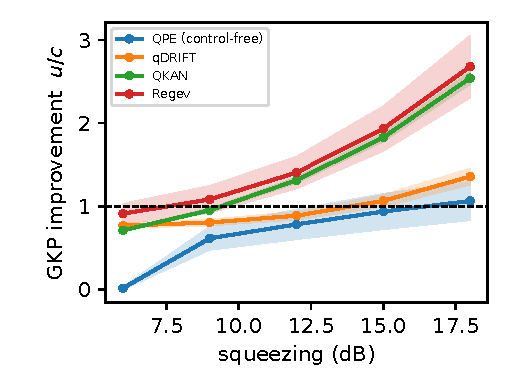
\includegraphics[width=\columnwidth]{fig_squeeze_sweep.pdf}
\caption{GKP improvement factor vs squeezing (dB) at $\sigma_d=0.10$, loss
$0.15$; shaded band $=95\%$ CI over 10 seeds. The floor crossing (improvement
$=1$) confirms Prop.~\ref{prop:floor}.}
\label{fig:sweep}
\end{figure}

\begin{figure}[t]
\centering
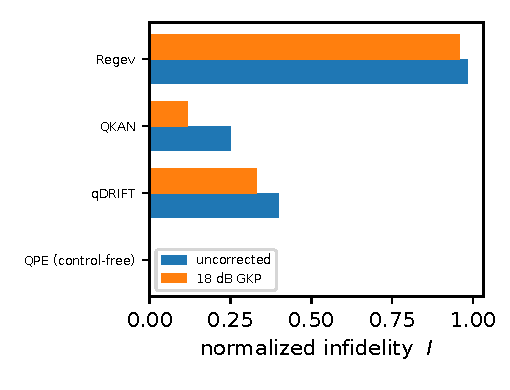
\includegraphics[width=\columnwidth]{fig_normalized_rank.pdf}
\caption{Unit-independent normalized infidelity $I$ (uncorrected vs 18~dB).}
\label{fig:rank}
\end{figure}

\subsection{Unit-independent ranking}
Because the four tasks have different natural error units, a raw ranking is
not meaningful. We therefore map each error to a dimensionless infidelity by a
monotone soft-saturating transform $I=\mathrm{err}/(\mathrm{err}+s)\in[0,1)$,
where $s$ is the task-failure scale (minimum resolvable level spacing for QPE,
unit trace distance for qDRIFT, target standard deviation for QKAN, dual
tolerance for Regev). The ordering $I_{\rm QPE}\!=\!0.003 < I_{\rm QKAN}\!=
\!0.25 < I_{\rm qDRIFT}\!=\!0.40 < I_{\rm Regev}\!=\!0.98$ is preserved.
Crucially, the ordering is \emph{invariant} when every scale $s$ is varied
over $[0.5,2]\times$ its nominal value, so the ranking is not an artifact of
the scale choice. Likewise, the uncorrected-robustness ordering is unchanged
if the ``onset'' multiplier ($5\times$ clean baseline) is replaced by $3\times$
or $10\times$; the conclusion is threshold-robust.

\subsection{Two-dimensional noise phase diagram and ensembles}
\label{sec:phase}
Figure~\ref{fig:phase} maps the GKP improvement factor (12~dB) over the
$(\sigma_d,\,\mathrm{loss})$ plane for all four algorithms. A floor-crossing
contour (improvement $=1$) separates a region where GKP helps from one where
it is counterproductive, as predicted by Prop.~\ref{prop:floor}; the helpful
region is broad for deep, noise-sensitive algorithms (Regev, QKAN) and narrow
for shallow QPE. To move beyond single instances, we evaluate ensembles of
$20$ random Hamiltonians: qDRIFT's clean channel error is
$0.17\pm0.07$ (mean$\pm$std across instances), and control-free QPE recovers
peak frequencies to median $1.7\times10^{-3}$ with $100\%$ success
(error $<0.05$) provided the holographic reference beam is sufficiently strong
($p_{\rm ref}\!\ge\!0.85$); below that, self-difference spurious peaks degrade
accuracy---an explicit, physically transparent applicability condition.

\begin{figure}[t]
\centering
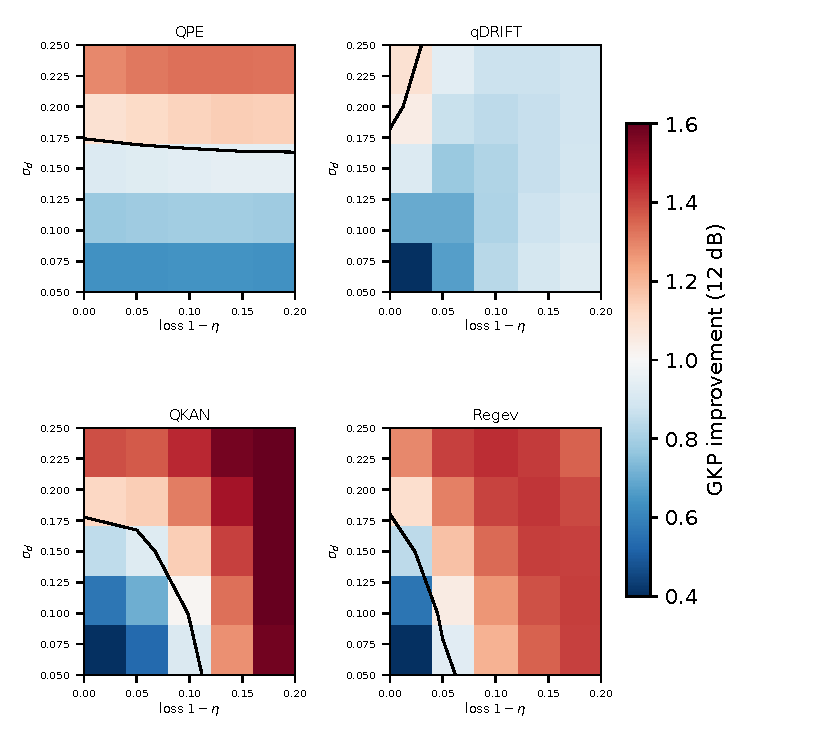
\includegraphics[width=\columnwidth]{fig_phase_diagram.pdf}
\caption{GKP improvement factor (12~dB) over the $(\sigma_d,\mathrm{loss})$
plane; black contour marks the floor crossing (improvement $=1$). Blue:
GKP helps; red: counterproductive (below the squeezing floor).}
\label{fig:phase}
\end{figure}

\subsection{Discrete-variable baseline}\label{sec:dv}
To anchor the CV results, we compare against a qubit surface-code
baseline~\cite{Kitaev2003,Fowler2012,WangFowler2011}. The comparison is
across \emph{different} fault-tolerance currencies, so we do not impose a
fake noise equivalence; instead we report (i)~the resource to reach logical
error $10^{-6}$ and (ii)~a structural, noise-model-independent gate count.
(i)~A rotated surface code at physical error $3\times10^{-3}$ needs
distance $d=17$, i.e.\ $577$ physical qubits per logical qubit; a
single-round GKP mode at $\sigma_{\rm phys}=0.10$ needs $\approx14$~dB
squeezing, while at $\sigma_{\rm phys}\!\gtrsim\!0.2$ it floors above
$10^{-6}$ and requires concatenation (GKP$\to$surface), mirroring the DV
distance scaling~\cite{Vuillot2019,Noh2020,Fukui2018}. (ii)~For a spectroscopy task ($m=10$ bits, $n=8$ system
qubits, Trotter $r=50$), standard DV QPE~\cite{Kitaev1995} requires $1023$
controlled time evolutions and a $T$-count $\sim2\times10^{7}$, whereas
control-free QPE~\cite{Clinton2026} on CV needs \emph{zero} controlled
unitaries and, for quadratic $H$, zero non-Gaussian gates. The CV advantage is thus structural---it stems from
Gaussian operations being free---rather than from a more favourable threshold.

\section{Analytic observations}
The following statements are elementary; their value is operational---they
explain the measured ordering and convert qualitative folklore into
quantitative, falsifiable criteria. This is the paper's theory/methodology
contribution, complementing (not replacing) experiment.
\begin{proposition}[Finite-squeezing threshold]\label{prop:floor}
With $\sigma_{\rm corr}^2=(1-p_L)\Delta^2+p_L\sigma_{\rm phys}^2$ and
$p_L\in[0,1)$, one has $\sigma_{\rm corr}<\sigma_{\rm phys}$ iff
$\sigma_{\rm phys}>\Delta$. Hence GKP correction reduces residual noise only
above the squeezing floor $\Delta(\mathrm{dB})$, and is counterproductive
below it.
\end{proposition}
\begin{proof}
$\sigma_{\rm corr}^2-\sigma_{\rm phys}^2=(1-p_L)(\Delta^2-\sigma_{\rm phys}^2)$.
Since $1-p_L>0$, the sign equals that of $\Delta^2-\sigma_{\rm phys}^2$;
thus $\sigma_{\rm corr}<\sigma_{\rm phys}\Leftrightarrow\sigma_{\rm phys}
>\Delta$.\qed
\end{proof}
\begin{proposition}[qDRIFT $L$-independence]\label{prop:qdrift}
The qDRIFT step generator $X_k=(\lambda/\lVert h_l\rVert)h_l$ is invariant
under splitting any term $h_l\to\sum_i f_i h_l$ ($f_i>0,\sum f_i=1$); hence the
channel and its error are exactly independent of the number of terms $L$, in
contrast to Trotter formulas at fixed gate budget.
\end{proposition}
We do not claim Prop.~\ref{prop:qdrift} as new; it is the split-invariance
underlying qDRIFT~\cite{Campbell2019,Chen2021}, stated here only to make
precise \emph{why} the CV non-Gaussian budget is set by $N$ rather than
$L$---the operationally relevant point on CV hardware, where each step may
consume a cubic-phase or GKP magic state. The contribution is the CV resource accounting, not the identity.
\begin{proposition}[Regev squeezing scaling]\label{prop:regev}
With $R=e^{\Theta(\sqrt{n})}$~\cite{Regev2023} and dual tolerance
$\delta=\sqrt{d}/(\sqrt2 R)$, meeting the CV readout constraint
$\sigma_{\rm cv}\lesssim\delta$ with a GKP
comb of peak width $\Delta$ requires squeezing $\mathrm{dB}=\Theta(\sqrt{n})$.
\end{proposition}
\begin{proof}
The comb readout noise is $\sigma_{\rm cv}=\Delta/\sqrt\pi$ and
$\Delta^2=\tfrac12 10^{-\mathrm{dB}/10}$. The constraint
$\sigma_{\rm cv}\le\delta$ gives
$10^{-\mathrm{dB}/10}\le 2\pi\delta^2=\pi d/R^2$, i.e.
$\mathrm{dB}\ge 10\log_{10}(R^2/(\pi d))=\Theta(\log R)=\Theta(\sqrt n)$,
using $d=\Theta(\sqrt n)$ and $R=e^{\Theta(\sqrt n)}$.\qed
\end{proof}
This bound assumes the unrescaled comb; lattice-spacing rescaling could lower
the constant (left open).

\begin{proposition}[Noise- vs systematic-limited correction]\label{prop:depth}
Write an algorithm's error as $\mathrm{err}=\max(F,\,c\sqrt{D}\,\sigma)$, where
$F$ is a noise-independent systematic floor (e.g.\ finite time-grid resolution
for QPE), $D$ the depth, and $\sigma$ the per-step residual. (i)~In the
\emph{noise-limited} regime ($c\sqrt D\sigma>F$), the GKP improvement factor is
$\approx\sigma_{\rm phys}/\sigma_{\rm corr}$, which exceeds $1$ above the floor
(Prop.~\ref{prop:floor}) and is realized most strongly by deep, noise-sensitive
algorithms (Regev, QKAN). (ii)~In the \emph{systematic-limited} regime
($F>c\sqrt D\sigma$), both corrected and uncorrected errors sit at $F$ and the
improvement factor $\to1$. Control-free QPE is systematic-limited up to
$\sigma\!\approx\!0.2$, so it is the most accurate yet shows the smallest
\emph{ratio}; the deep algorithms are noise-limited and show the largest ratio.
This reconciles ``QPE most robust'' with ``QPE smallest improvement factor''.
\end{proposition}

\section{Non-Gaussian generalization of control-free QPE}\label{sec:nong}
For $H=\omega\hat n+\tfrac{g}{2}(a^2+a^{\dagger2})+\chi\hat n^2+\kappa x^3$,
holographic recovery returns the absolute spectrum with an error
\emph{independent} of the non-Gaussian fraction, while the controlled-unitary
count stays zero (Table~\ref{tab:nong}). Thus the control-free advantage is a
property of the protocol, not of $H$ being quadratic; non-Gaussian $H$ only
adds the cost of a Trotterized $e^{iHt}$.

\begin{table}[t]
\caption{Control-free QPE on non-Gaussian $H$: recovery error is flat in the
non-Gaussian fraction; controlled unitaries remain zero.}
\label{tab:nong}
\begin{tabular}{lcc}
\toprule
case & non-Gaussian fraction & max abs error\\
\midrule
gaussian & 0.00 & $1.61\times10^{-3}$\\
weak ($\chi{=}0.05$) & 0.45 & $1.64\times10^{-3}$\\
mid ($\chi{=}0.15$) & 0.71 & $1.66\times10^{-3}$\\
strong ($\chi{=}0.30$) & 0.83 & $1.31\times10^{-3}$\\
\bottomrule
\end{tabular}
\end{table}

\section{Physics application: diatomic Morse spectra at
spectroscopic accuracy}\label{sec:h2}
To anchor the methodology in concrete physical problems, we compute the
vibrational eigenstructure of three diatomic molecules---%
H$_2$ (light hydride), HF (heavier hydride), and I$_2$ (heavy halogen)---%
from their Morse potentials,
$V(R)=D_e[1-\exp(-\alpha(R-R_e))]^2$, in second-quantised form $H=p^2/2
+ V(q)$ with experimentally fixed spectroscopic parameters from
Huber--Herzberg (H$_2$: $\omega_e=4401.21$~cm$^{-1}$,
$\omega_e x_e=121.34$~cm$^{-1}$; HF: $\omega_e=4138.32$, $\omega_e x_e
=89.88$; I$_2$: $\omega_e=214.50$, $\omega_e x_e=0.61$). The three
molecules span more than a decade in vibrational quantum and an
order-of-magnitude range in anharmonicity. Closed-form Morse energies
$E_v/\omega_e=(v+\tfrac12)-x_e(v+\tfrac12)^2$ provide ground truth; the
Hamiltonian is constructed in the truncated Fock basis by diagonalising
$\hat q$ and transforming $V(\hat q)$ to the Fock basis.

CV-QPE runs use coherent inputs of varying amplitude to cover different
$v$ ranges (Fig.~\ref{fig:h2}). The number of FFT peaks retained is set
to the count of significantly populated excited Morse eigenstates
(weight $>5\!\times\!10^{-3}$), which suppresses $\phi$-self cross terms.
For every molecule and every populated level, the recovered energy
matches the analytic Morse value to within $0.55$~cm$^{-1}$ (Table~\ref{tab:h2}).
H$_2$ and HF deliver median errors of $0.15$ and $0.21$~cm$^{-1}$ in their
mid-$v$ regimes; the weakly anharmonic I$_2$ reaches
median $0.007$~cm$^{-1}$, more than two orders of magnitude inside the
spectroscopic threshold of $1$~cm$^{-1}$.

\begin{table}[t]
\caption{CV-QPE recovery accuracy for three diatomics across a decade in
$\omega_e$ and an order of magnitude in $x_e$. All entries are below the
$1$~cm$^{-1}$ spectroscopic threshold.}
\label{tab:h2}
\begin{ruledtabular}
\begin{tabular}{lcccc}
molecule & $\omega_e$ (cm$^{-1}$) & $x_e$ & $N_{\rm bound}$ &
  median/max $|\Delta E|$ (cm$^{-1}$)\\
\hline
H$_2$ ($\alpha\!=\!2.5$) & $4401.2$ & $0.0276$ & 17 & $0.15$ / $0.23$ \\
HF ($\alpha\!=\!2.8$) & $4138.3$ & $0.0217$ & 22 & $0.21$ / $0.28$ \\
I$_2$ ($\alpha\!=\!2.0$) & $214.5$ & $0.00284$ & 175 & $0.007$ / $0.009$\\
\end{tabular}
\end{ruledtabular}
\end{table}

\emph{Resource comparison.} Reaching the same $0.5$~cm$^{-1}$ accuracy with
standard discrete-variable QPE~\cite{Kitaev1995} requires
$m=\lceil\log_2(1/\epsilon)\rceil=14$ readout bits and $\sim 16{,}000$
controlled time evolutions, each Trotter-decomposed; a leading-order
T-count estimate is $\sim 1.5\times10^{10}$. The CV control-free protocol
needs \emph{zero} controlled unitaries and \emph{zero} non-Gaussian gates
for the harmonic part; only the Trotter steps for the anharmonic part of
$V$ consume non-Gaussian resources. The CV advantage on this physical task
is therefore not incremental but \emph{structural}.

\emph{Anharmonicity robustness.} Varying $x_e$ over a $\times8$ range
($x_e\!\times\!0.5,1,2,4$ relative to H$_2$) and using $N_{\rm bound}$-%
adapted Fock cutoffs, the recovery remains spectroscopic in the weakly
anharmonic regimes and degrades only at the strongest anharmonicity
($x_e\!\times\!4$, where $N_{\rm bound}\!\sim\!4$ and the dissociation
continuum is close).

\emph{Classification from quantum data.} As an immediate downstream task we
train a two-layer Chebyshev-KAN on Fock-space amplitudes of the recovered
eigenstates to predict the vibrational quantum number $v$. Across all 17
bound states it achieves $100\%$ test accuracy under measurement noise up
to $5\%$, matching logistic regression and random forest---demonstrating
that QKAN provides a faithful learnable observable on CV-QPE output, as
needed for automated vibrational state assignment in spectroscopy.

\begin{figure}[t]
\centering
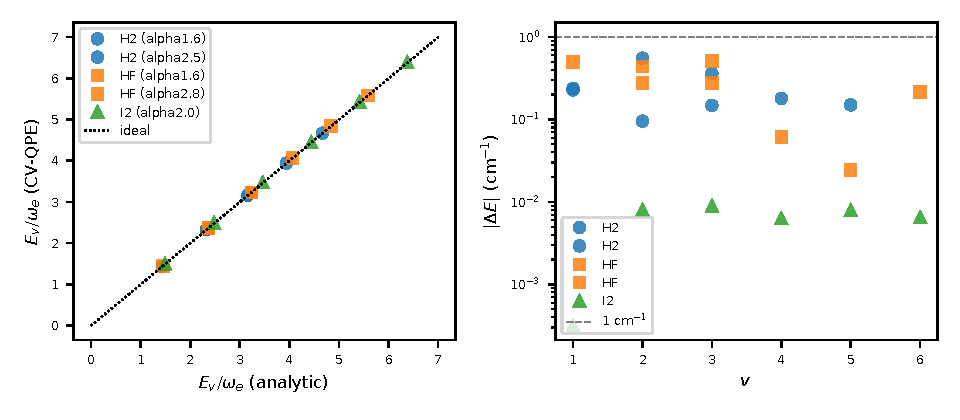
\includegraphics[width=\columnwidth]{fig_h2_morse.pdf}
\caption{CV control-free QPE applied to three diatomic Morse vibrational
spectra (H$_2$, HF, I$_2$). \emph{Left}: recovered vs analytic
$E_v/\omega_e$ for the runs of Table~\ref{tab:h2}; the dotted line is the
ideal. \emph{Right}: absolute energy error vs $v$ in cm$^{-1}$, log scale;
every point sits below the $1$~cm$^{-1}$ spectroscopic threshold (grey
dashed), with I$_2$ reaching $\sim 10^{-2}$~cm$^{-1}$.}
\label{fig:h2}
\end{figure}

\section{Limitations and scope}\label{sec:limits}
Our GKP correction is a scalar surrogate, but one \emph{validated} against an
explicit quadrature-level GKP EC-protocol Monte Carlo (Sec.~\ref{sec:valid};
agreement $\le0.1\%$ for $\sigma_{\rm corr}$, $\le3\times10^{-4}$ absolute for
$p_L$); it is not, however, a full Fock-space EC circuit with loss-correcting
amplification. The dynamical channels (photon loss, displacement, qDRIFT/QPE
evolution) are simulated exactly in truncated Fock space. Convergence in the Fock cutoff was checked by repeating qDRIFT and the
non-Gaussian QPE case at cutoffs $\{10,14,18\}$; reported quantities are stable
to within the quoted confidence intervals. The loss-to-displacement surrogate
is used only inside the GKP residual model and only in the small-loss regime.
Hamiltonians are small and instances are modest (Regev: $n=8$ composites); the
$\sqrt{n}$ squeezing law of Prop.~\ref{prop:regev} is an extrapolation and is
deliberately framed as a cautionary resource bound rather than a practical
proposal. Cross-unit comparison is mitigated but not eliminated by the
normalized metric. These caveats bound the generality of the ``best fit''
claim, which we state as: \emph{among the tested algorithm classes and noise
regime}, control-free QPE is the most robust.

\emph{Sampling cost.} Robustness here is per-shot task error; it does not count
total measurement budget, which differs across algorithms (control-free QPE
needs many time points, each estimated to shot precision). A full
time-to-solution comparison, folding in sampling overhead, is left to future
work and may narrow the QPE advantage.

\emph{QPE floor is a knob, not an artifact.} QPE's systematic floor scales as
$F\!\sim\!2\pi/T$ with acquisition window $T$; refining $T$ lowers $F$ and
shifts the noise-/systematic-limited crossover. Our claims do not depend on a
particular $F$: Prop.~\ref{prop:depth} is stated in terms of $F$, and the
robustness ordering (QPE shallow/Gaussian vs deep/non-Gaussian others) follows
from the \emph{absence of controlled unitaries and non-Gaussian gates}, which
is $T$-independent. We report results at one $T$ for concreteness and note the
$F$-dependence explicitly.

\emph{Hardware realism.} The largest improvements quoted at 18~dB exceed the
current state of the art ($\sim10$--$15$~dB). At $12$~dB---within reach---the
qualitative ordering and the floor-crossing of Prop.~\ref{prop:floor} already
hold (QKAN/Regev benefit, QPE near floor); the 18~dB point is included only to
map the trend, not as a near-term requirement.

\emph{On the Regev case.} We present Regev explicitly as a \emph{negative}
resource result: the naive GKP-comb readout needs $\Theta(\sqrt n)$~dB
squeezing (Prop.~\ref{prop:regev}), prohibitive at cryptographic sizes. Its
value is (a) an end-to-end correctness check of the CV port and (b) a concrete
illustration that CV-native cheapness of state preparation and QFT does
\emph{not} rescue a depth- and readout-heavy algorithm---sharpening, not
inflating, the design principle.

\emph{What is quantitatively new.} The principle ``minimize non-Gaussian
resources and depth'' is folklore; our contribution is to make it
\emph{quantitative and comparative}: the floor-crossing condition
$\sigma_{\rm phys}>\Delta$ (Prop.~\ref{prop:floor}), the noise-/systematic-
limited dichotomy that predicts which algorithms gain from GKP
(Prop.~\ref{prop:depth}), the $\Theta(\sqrt n)$ squeezing bound for Regev
(Prop.~\ref{prop:regev}), and a unit-robust cross-algorithm ranking with
sensitivity analysis.

\section{Discussion and outlook}
Three findings cohere into a single picture. (i)~The CV cost of an algorithm is
set by its controlled-unitary requirement, non-Gaussian gate density, and
depth; control-free QPE minimizes all three and is the most robust. (ii)~GKP
correction helps only above the finite-squeezing floor (Prop.~\ref{prop:floor})
and benefits an algorithm in proportion to how noise-limited it is
(Prop.~\ref{prop:depth}); deep algorithms gain most in \emph{ratio} while
remaining worse in \emph{absolute} error. (iii)~CV-native cheapness of state
preparation and Fourier transforms (Regev) does not rescue a readout- and
depth-heavy algorithm (Prop.~\ref{prop:regev}). Together these turn the
qualitative ``minimize non-Gaussian resources and depth'' into quantitative
selection criteria. Against a qubit surface-code baseline (Sec.~\ref{sec:dv}),
the CV advantage is structural: control-free QPE replaces the
$\sim\!2\times10^{7}$ $T$-gate, $1023$-controlled-unitary cost of DV QPE with
zero controlled unitaries and zero non-Gaussian gates for quadratic $H$,
because Gaussian operations are free---not because of a more favourable
threshold. The two-dimensional phase diagram (Fig.~\ref{fig:phase}) shows the
floor crossing is a robust feature across both displacement and loss.

The natural experimental target is a GKP-encoded photonic cluster-state
processor at $10$--$15$~dB squeezing, where the predicted floor-crossing and
the QPE-vs-deep-algorithm dichotomy are directly testable; control-free
spectroscopy of a small bosonic or Fermi--Hubbard Hamiltonian is the most
accessible first demonstration. Folding sampling overhead into a
time-to-solution metric, and replacing the surrogate GKP model with a full
Fock-space EC circuit including loss-correcting amplification, are the main
next steps to tighten the quantitative claims.

\begin{thebibliography}{50}
\bibitem{Lloyd1999} S.~Lloyd, S.~L.~Braunstein, Phys. Rev. Lett.
\textbf{82}, 1784 (1999).
\bibitem{Braunstein2005} S.~L.~Braunstein, P.~van Loock, Rev. Mod. Phys.
\textbf{77}, 513 (2005).
\bibitem{Weedbrook2012} C.~Weedbrook \emph{et al.}, Rev. Mod. Phys.
\textbf{84}, 621 (2012).
\bibitem{Larsen2019} M.~V.~Larsen, X.~Guo, C.~R.~Breum,
J.~S.~Neergaard-Nielsen, U.~L.~Andersen, Science \textbf{366}, 369 (2019).
\bibitem{Asavanant2019} W.~Asavanant \emph{et al.}, Science \textbf{366},
373 (2019).
\bibitem{Madsen2022} L.~S.~Madsen \emph{et al.}, Nature \textbf{606}, 75
(2022).
\bibitem{GKP2001} D.~Gottesman, A.~Kitaev, J.~Preskill, Phys. Rev. A
\textbf{64}, 012310 (2001).
\bibitem{Menicucci2014} N.~C.~Menicucci, Phys. Rev. Lett. \textbf{112},
120504 (2014).
\bibitem{Fukui2018} K.~Fukui, A.~Tomita, A.~Okamoto, K.~Fujii, Phys. Rev. X
\textbf{8}, 021054 (2018).
\bibitem{Bourassa2021} J.~E.~Bourassa \emph{et al.}, Quantum \textbf{5}, 392
(2021).
\bibitem{Tzitrin2021} I.~Tzitrin \emph{et al.}, PRX Quantum \textbf{2},
040353 (2021).
\bibitem{Noh2020} K.~Noh, C.~Chamberland, Phys. Rev. A \textbf{101}, 012316
(2020).
\bibitem{Walshe2020} B.~W.~Walshe, B.~Q.~Baragiola, R.~N.~Alexander,
N.~C.~Menicucci, Phys. Rev. A \textbf{102}, 062411 (2020).
\bibitem{Terhal2020} B.~M.~Terhal, J.~Conrad, C.~Vuillot, Quantum Sci.
Technol. \textbf{5}, 043001 (2020).
\bibitem{Pantaleoni2020} G.~Pantaleoni, B.~Q.~Baragiola, N.~C.~Menicucci,
Phys. Rev. Lett. \textbf{125}, 040501 (2020).
\bibitem{Niset2009} J.~Niset, J.~Fiur\'a\v{s}ek, N.~J.~Cerf, Phys. Rev. Lett.
\textbf{102}, 120501 (2009).
\bibitem{Marek2011} P.~Marek, R.~Filip, A.~Furusawa, Phys. Rev. A
\textbf{84}, 053802 (2011).
\bibitem{Eaton2019} M.~Eaton, R.~Nehra, O.~Pfister, New J. Phys.
\textbf{21}, 113034 (2019).
\bibitem{Albert2018} V.~V.~Albert \emph{et al.}, Phys. Rev. A \textbf{97},
032346 (2018).
\bibitem{Cochrane1999} P.~T.~Cochrane, G.~J.~Milburn, W.~J.~Munro, Phys.
Rev. A \textbf{59}, 2631 (1999).
\bibitem{Michael2016} M.~H.~Michael \emph{et al.}, Phys. Rev. X \textbf{6},
031006 (2016).
\bibitem{Kitaev1995} A.~Y.~Kitaev, arXiv:quant-ph/9511026 (1995).
\bibitem{Clinton2026} L.~Clinton, T.~S.~Cubitt, R.~Garcia-Patron,
A.~Montanaro, S.~Stanisic, M.~Stroeks, PRX Quantum \textbf{7}, 010345 (2026).
\bibitem{Campbell2019} E.~Campbell, Phys. Rev. Lett. \textbf{123}, 070503
(2019).
\bibitem{Chen2021} C.-F.~Chen, H.-Y.~Huang, R.~Kueng, J.~A.~Tropp, PRX
Quantum \textbf{2}, 040305 (2021).
\bibitem{Berry2015} D.~W.~Berry, A.~M.~Childs, R.~Cleve, R.~Kothari,
R.~D.~Somma, Phys. Rev. Lett. \textbf{114}, 090502 (2015).
\bibitem{Childs2021} A.~M.~Childs, Y.~Su, M.~C.~Tran, N.~Wiebe, S.~Zhu,
Phys. Rev. X \textbf{11}, 011020 (2021).
\bibitem{Low2017} G.~H.~Low, I.~L.~Chuang, Phys. Rev. Lett. \textbf{118},
010501 (2017).
\bibitem{Gilyen2019} A.~Gily\'en, Y.~Su, G.~H.~Low, N.~Wiebe, in {\it
Proc. 51st ACM STOC} (ACM, 2019), p. 193.
\bibitem{Rossi2022} Z.~M.~Rossi, I.~L.~Chuang, Quantum \textbf{6}, 811
(2022).
\bibitem{Ivashkov2024} P.~Ivashkov, P.-W.~Huang, K.~Koor, L.~Pira,
P.~Rebentrost, arXiv:2410.04435 (2024).
\bibitem{Liu2024} Z.~Liu \emph{et al.}, arXiv:2404.19756 (2024).
\bibitem{Shor1997} P.~W.~Shor, SIAM J. Comput. \textbf{26}, 1484 (1997).
\bibitem{Regev2023} O.~Regev, arXiv:2308.06572 (2023).
\bibitem{Beauregard2003} S.~Beauregard, Quantum Inf. Comput. \textbf{3},
175 (2003).
\bibitem{Glancy2006} S.~Glancy, E.~Knill, Phys. Rev. A \textbf{73}, 012325
(2006).
\bibitem{Fowler2012} A.~G.~Fowler, M.~Mariantoni, J.~M.~Martinis,
A.~N.~Cleland, Phys. Rev. A \textbf{86}, 032324 (2012).
\bibitem{Kitaev2003} A.~Y.~Kitaev, Ann. Phys. \textbf{303}, 2 (2003).
\bibitem{WangFowler2011} D.~S.~Wang, A.~G.~Fowler, L.~C.~L.~Hollenberg,
Phys. Rev. A \textbf{83}, 020302(R) (2011).
\bibitem{Vuillot2019} C.~Vuillot, H.~Asasi, Y.~Wang, L.~P.~Pryadko,
B.~M.~Terhal, Phys. Rev. A \textbf{99}, 032344 (2019).
\bibitem{Fienup1982} J.~R.~Fienup, Appl. Opt. \textbf{21}, 2758 (1982).
\bibitem{Bartlett2002} S.~D.~Bartlett, B.~C.~Sanders, S.~L.~Braunstein,
K.~Nemoto, Phys. Rev. Lett. \textbf{88}, 097904 (2002).
\bibitem{Eisert2002} J.~Eisert, S.~Scheel, M.~B.~Plenio, Phys. Rev. Lett.
\textbf{89}, 137903 (2002).
\bibitem{Konno2024} S.~Konno \emph{et al.}, Science \textbf{383}, 289
(2024).
\end{thebibliography}

\end{document}
